\section{\textit{Backend} \textit{Django}}
Esta sessão tratará sobre o servidor do sistema, também conhecido como \textit{backend}
ou \textit{API} \textit{Django}. Na primeira subsessão, é tratada uma breve descrição sobre as funções
e características deste. A segunda apresenta o \textit{design} e a arquitetura
de desenvolvimento. Por fim, trataremos as instâncias do projeto desenvolvido.


\subsection{Papel do \textit{Backend}}
\label{sub:papel_da_api}
O \textit{backend} do sistema, responsável por fazer o controle das requisições,
atuando como intermediador à cadeira e aos seus respectivos monitores
foi desenvolvida utilizando o \textit{Django Rest Framework}, que é uma
referência no mundo de desenvolvimento de API's para \textit{Python}.

O \textit{backend} manipula todos os dados enviados pela cadeira, utilizando a \textit{Raspberry}
executa o processamento desses dados e envia notificações para os \textit{smartphones}
cadastrados no sistema. Além disso, serve dados para uma interface web de controle
do monitor.

A manipulação dos dados é feita de forma segura, tratando a autenticação dos usuários
que lidam com o sistema e redirecionando os dados de acordo com a sua autenticação.
Para a execução dos passos, o servidor conta com um poderoso sistema de autenticação
dos seus usuários, tanto para os pacientes que utilizam a cadeira, quanto para os
monitores que manipulam as interfaces para cliente, como mobile e interface web.
Os pacientes são cadastrados no sistema e enviam os sinais corporais para o servidor.
O servidor, além de enviar uma notificação para o monitor respectivo, armazena este
sinal em sua base de dados e retorna ao monitor quando solicitado.
Os dados enviados ao monitor são apenas os sinais respectivos ao paciente que está
sendo monitorado.

A ligação entre o paciente e o monitor pode ser feita no momento do cadastro ou em
atualizações futuras. O paciente contém um identificador único em sua cadeira, que
pode ser utilizado pelo monitor para supervisioná-lo. No momento que o monitor insere
os dados no sistema, automaticamente será ligado ao paciente e terá acesso aos dados
de sinais enviados pelo paciente.

\subsection{\textit{Design} e Arquitetura da Solução}
\label{sub:design_e_arquitetura_da_soluca_o}

O \textit{django} utiliza de uma arquitetura própria para padronização e aplicação de boas
práticas em desenvolvimento de \textit{API}'s. Esta arquitetura está dividida em \textit{tiers},
que são responsáveis por funções específicas e cada uma tem seu papel definido
para a manipulação de dados no sistema. A seguir está uma ilustração do funcionamento
da arquitetura do servidor.

\begin{figure}
    \begin{center}
        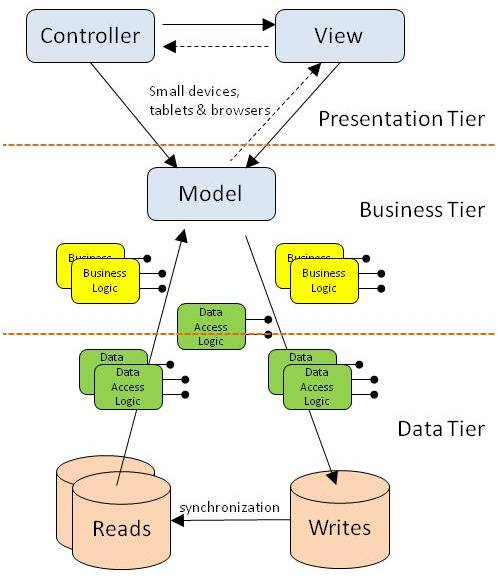
\includegraphics[scale=0.6]{figuras/rest_arch.jpg}
    \end{center}
    \caption{\textit{Design} e Arquitetura do servidor \textit{Django} \cite{serveruml}}
    \label{fig:rest_arch}
\end{figure}

Como pode ser observado, existem três \textit{Tiers} principais, que são utilizadas
para a manipulação dos dados. Elas são:

\begin{itemize}
    \item \textit{Presentation Tier;}
    \item \textit{Business Tier;}
    \item \textit{Data Tier.}
\end{itemize}

A primeira, \textit{Presentation Tier} é responsável por ser a interface com as demais aplicações
que irão utilizar o servidor. Essa \textit{tier} é responsável por gerir as rotas do sistema, direcionando
as urls solicitadas a funções específicas. Após mapeado nas funções, estas irão verificar as permissões
de cada requisição, bem como cada usuário que está solicitando uma determinada ação.

Além disso, nesta \textit{tier}, existe uma transformação importante para o consumo de dados por parte dos clientes.
Esta é conhecida como serialização dos dados, tanto para quem envia, quanto para quem solicita.
Sua responsabilidade é aplicar um modelo de dados formalizado na comunidade, conhecido como \textit{json}.
Dessa forma, todo tipo de dado recebido, assim como os enviados são transformados  a partir
dos objetos \textit{Python}. Esta fase é aplicada logo após a aplicação das rotas para as respectivas
ações.

As funções mapeadas na \textit{Tier} passada utiliza de modelos predefinidos na Business \textit{Tier}.
Aqui são definidos os domínios da aplicação, bem como quais são as classes e negócio da
aplicação. Nesta fase são definidos os tipos de usuários do sistema, as classes de sinais
corporais do paciente e toda parte  de negócios da aplicação.

A última \textit{tier}, chamada de \textit{Data Tier} é responsável por lidar com a persistência dos dados
de todos os usuários e sinais que são manipulados no sistema. Esta  \textit{tier}  modela o
bando de dados assim como foi definido na aplicação de negócios e aplica
inserções neste a medida que novas requisições são feitas.

\subsection{Projeto Desenvolvido}
\label{sub:projetodesenvolvido}

O projeto UMISS-BackEnd, desenvolvido exatamente na arquitetura apresentada na sessão
\ref{sub:design_e_arquitetura_da_soluca_o}, possui entidades que deram formato à Business
\textit{Tier} do projeto, onde são definidas as propriedades do sistema, bem como ele atuará.

No projeto, foi desenvolvido o diagrama de classes, que auxilia na atividade de compreender
o domínio do projeto. Este está no Anexo \ref{anx:server_uml}.

É possível visualizar que existem várias entidades de usuários. Isto foi desenvolvido pois
existem dois tipos de usuários diferentes no sistema. Eles são o Paciente e o Monitor. Estes
possuem atributos e comportamentos diferentes, gerando assim a necessidade de implementação
de dois domínios diferentes.  Da mesma maneira, existem três tipos de sinais corporais que são enviados pelo paciente.
Esses sinais possuem características diferentes, bem como atributos. Dessa maneira, existe
uma entidade generalista chamada \textit{BodySignal} com características comuns de todas. E
foram criados as demais especializações com suas características  específicas. Elas são:
Sinais de temperatura corporal, Sinais de batimento cardíaco e Sinais de resistência galvânica.

Por fim, existem ligações dos usuários com os sinais corporais, sendo que os pacientes
são donos destes. Assim como exitem pacientes que possuem monitores ligados,
gerando um relacionamento cíclico entre as entidades de usuário.
